\subsubsection{Группа}
    Рассмотрим некоторую группу $G$, ее фактор-группу $G/G'$ по коммутанту 
    $G'$ и следующую диаграмму

    \begin{figure}[h]
        \centering
        \[\xymatrix{
            G \ar[rr]^{\textstyle{\tau}} \ar[rrdd]_{\textstyle{\chi}} & & G/G'\ar[dd]^{\textstyle{\chi_{ab}}} \\
            & & \\
            & & \mathbb{C}
        }\]
        \caption{}
        \label{cd_ab}
    \end{figure}

    Здесь $\tau: g \mapsto gG'$ --- канонический гомоморфизм; $\chi$, 
    $\chi_{ab}$ --- характеры групп $G$ и $G/G'$ соответственно.

    Оказывается, что 

    \begin{lemma}\label{lm_const} Для любых $f, g \in G$, таких что $f = g \mod G'$ 
        \[\chi(f) = \chi(g).\]
    \end{lemma}

    \begin{proof} Действительно, в условиях леммы существует $h \in G'$, 
        такой что $f = gh$, но по определению коммутанта существуют такие 
        $a$ и $b$, что $h = aba^{-1}b^{-1}$, откуда $f = gaba^{-1}b^{-1}$, и 
        \[\chi(f) = \chi(gaba^{-1}b^{-1}) 
        = \chi(g) + \chi(a) + \chi(b) - \chi(a) - \chi(b) = \chi(g).\]
    \end{proof}

    Иными словами доказано, что факторизация 
    группы по коммутанту $G'$ разбивает ее на области постоянства
    характера (рис. \ref{img_chi_factor}). А значит вместо 
    рассмотрения характера $\chi$ на всей группе, достаточно пронаблюдать 
    лишь за его "<действием с точностью до $G'$">, т.е. за некоторым характером
    $\chi_{ab}$ на $G/G'$.

    \begin{figure}[h]
        \centering
        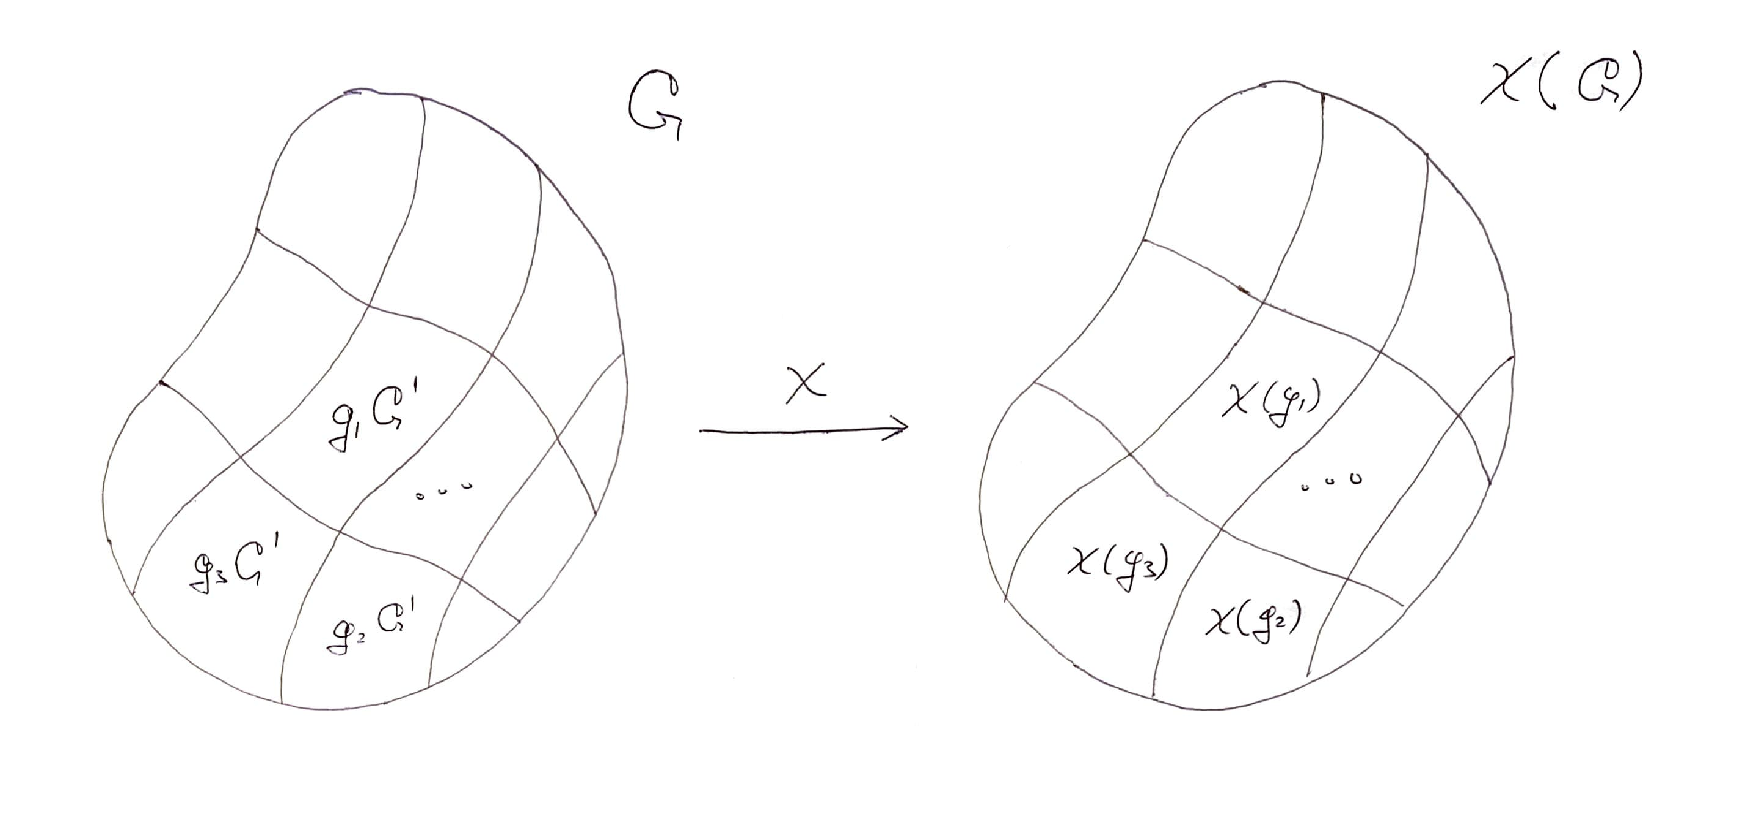
\includegraphics[width=\textwidth]{pictures/chips}
        \caption{}
        \label{img_chi_factor}
    \end{figure}

    Так, введем, очевидно инъективный, гомоморфизм 
    $t: X(G/G') \to X(G)$ пространств характеров:
    \begin{equation}
        t : \chi_{ab} \mapsto \chi_{ab} \circ \tau = \chi. 
    \end{equation}
    Его сюръективность вытекает напрямую из леммы \ref{lm_const}, ибо для 
    любого $\chi : G \to \mathbb{C}$ корректно задан $\chi_{ab}$:
    \[\chi_{ab}(gG') = \chi(g),\]
    который удовлетворяет 
    \[\chi_{ab} \circ \tau = \chi.\]
    Тем самым доказано
    \begin{statement}
        \[X(G) \simeq X(G/G'),\]
    \end{statement}
    Позволяющее задавать характер не на самой группе, а на ее 
    абелизации, что и приводит нас к следующему параграфу.
    